\subsection{Method evaluation} \label{meth-synth-method-subsect}
\emph{Fig. \ref{probit-2nd-pic}} depicts the three latent functions $\mathbf{f}$ that are fitted to the synthetic data after running the EM algorithm. The coloured data points show three regions from the whole dataset, chosen randomly after being assigned to one of the three clusters. It is evident that the fitted latent functions have recovered the procedure that generated the data. The latent functions are restricted to $2^{nd}$ degree polynomials.
\begin{figure}[!ht]
\begin{center}
 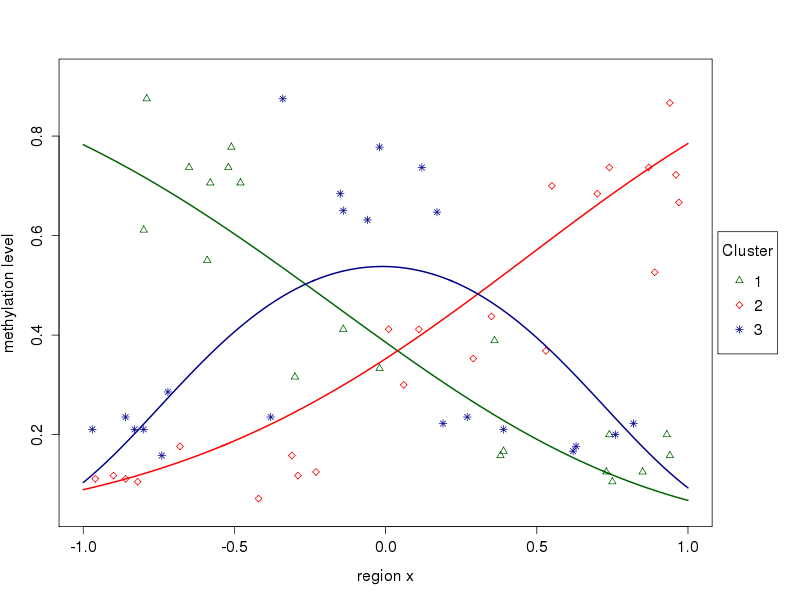
\includegraphics[scale = 0.40]{images/probit2nd.png}
\caption{\emph{Clustering DNA methylation profiles with $2^{nd}$ degree polynomial.}}
\label{probit-2nd-pic}
\end{center}
\end{figure}

\emph{Fig. \ref{probit-3rd-pic}} depicts the same regions as \emph{Fig. \ref{probit-2nd-pic}} above, but now the methylation profiles are modelled using $3^{rd}$ degree polynomial functions. It is clear that as we increase the degree of polynomials, the functions will be less restricted and can model better the methylation profiles, but care should be taken due to \emph{overfitting}.
\begin{figure}[!ht]
\begin{center}
 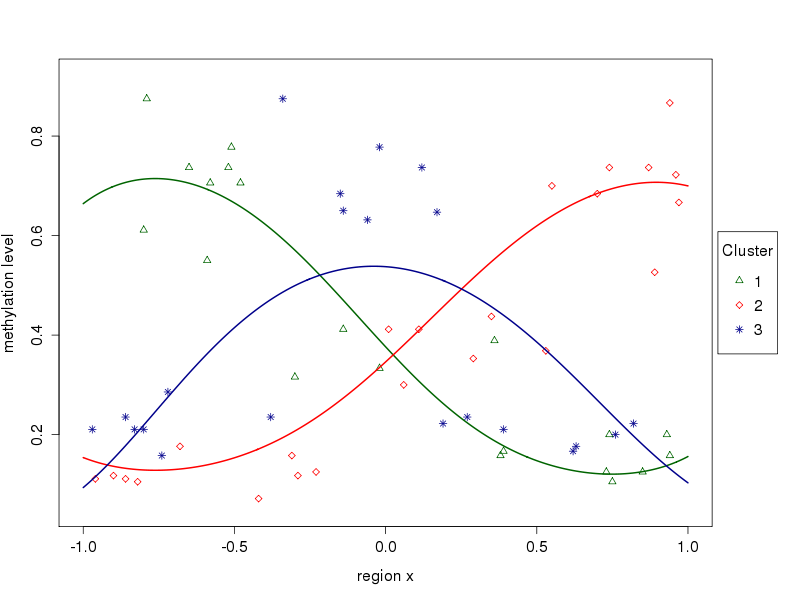
\includegraphics[scale = 0.40]{images/probit3rd.png}
\caption{\emph{Clustering DNA methylation profiles with $3^{rd}$ degree polynomial.}}
\label{probit-3rd-pic}
\end{center}
\end{figure}